\chapter{Trigonometria}

\begin{theorybox}{Trazabilidad del capitulo}
Este capitulo desarrolla las secciones \texttt{C05.S01-C05.S08} de la matriz de cobertura a
partir de \texttt{sources/Relacion tema 5.pdf}. El foco didactico es controlar unidades,
cuadrantes y elecciones de metodo antes de pasar a ecuaciones, triangulos y problemas de
contexto.
\end{theorybox}

\section{[C05.S01] Grados y radianes}

\subsection*{Objetivos de aprendizaje}
\begin{itemize}
  \item Convertir angulos de grados a radianes y viceversa.
  \item Reconocer equivalencias basicas entre vuelta, semivuelta y cuarto de vuelta.
\end{itemize}

\subsection*{Prerrequisitos}
\begin{itemize}
  \item Fracciones y proporcionalidad.
\end{itemize}

\begin{theorybox}{Idea minima}
Una vuelta completa mide \(360^\circ\) y tambien \(2\pi\) radianes. Por eso
\[
180^\circ=\pi \text{ rad},\qquad 1^\circ=\frac{\pi}{180}\text{ rad},\qquad
1\text{ rad}=\frac{180^\circ}{\pi}.
\]
\end{theorybox}

\begin{methodbox}{Como reconocer y resolver}
\begin{enumerate}
  \item Si partes de grados, multiplica por \(\frac{\pi}{180}\).
  \item Si partes de radianes, multiplica por \(\frac{180}{\pi}\).
  \item Simplifica la fraccion final si es posible.
\end{enumerate}
\end{methodbox}

\begin{solvedexample}{[EX-C05.S01-01] Convertir en ambos sentidos}
Convierte \(135^\circ\) a radianes y \(\frac{7\pi}{6}\) radianes a grados.

\textbf{Desarrollo.}
\[
135^\circ=\frac{135\pi}{180}=\frac{3\pi}{4}\text{ rad}.
\]
Para el segundo:
\[
\frac{7\pi}{6}\text{ rad}=\frac{7\pi}{6}\cdot \frac{180^\circ}{\pi}=210^\circ.
\]

\textbf{Respuesta final.}
\[
135^\circ=\frac{3\pi}{4}\text{ rad},
\qquad
\frac{7\pi}{6}\text{ rad}=210^\circ.
\]
\end{solvedexample}

\begin{commonerror}{Cancelar la \(\pi\) cuando no toca}
En una conversion de grados a radianes la \(\pi\) debe aparecer en el resultado. Si desaparece,
seguramente se ha usado la razon al reves.
\end{commonerror}

\begin{guidedexercise}{[GX-C05.S01-01] De grados a radianes}
Convierte \(210^\circ\) a radianes.

\textbf{Pista 1.} Multiplica por \(\frac{\pi}{180}\) y simplifica.
\end{guidedexercise}

\begin{shortanswer}{[GX-C05.S01-01]}
\[
210^\circ=\frac{7\pi}{6}\text{ rad}.
\]
\end{shortanswer}

\begin{fullsolution}{[GX-C05.S01-01]}
\[
210^\circ=\frac{210\pi}{180}=\frac{7\pi}{6}\text{ rad}.
\]
\end{fullsolution}

\begin{guidedexercise}{[GX-C05.S01-02] De radianes a grados}
Convierte \(\frac{3\pi}{4}\) radianes a grados.

\textbf{Pista 1.} Multiplica por \(\frac{180^\circ}{\pi}\).
\end{guidedexercise}

\begin{shortanswer}{[GX-C05.S01-02]}
\[
\frac{3\pi}{4}\text{ rad}=135^\circ.
\]
\end{shortanswer}

\begin{fullsolution}{[GX-C05.S01-02]}
\[
\frac{3\pi}{4}\cdot \frac{180^\circ}{\pi}=135^\circ.
\]
\end{fullsolution}

\subsection*{Practica autonoma graduada}
\begin{exercise}{[PX-C05.S01-01] Convierte \(30^\circ\) a radianes.}
\end{exercise}
\begin{exercise}{[PX-C05.S01-02] Convierte \(300^\circ\) a radianes.}
\end{exercise}
\begin{exercise}{[PX-C05.S01-03] Convierte \(\frac{\pi}{5}\) radianes a grados.}
\end{exercise}
\begin{exercise}{[PX-C05.S01-04] Convierte \(\frac{11\pi}{6}\) radianes a grados.}
\end{exercise}
\begin{exercise}{[PX-C05.S01-05] Convierte \(225^\circ\) a radianes.}
\end{exercise}
\begin{exercise}{[PX-C05.S01-06] Convierte \(\frac{2\pi}{3}\) radianes a grados.}
\end{exercise}

\begin{shortanswer}{C05.S01 practica autonoma}
\begin{enumerate}[label=\textbf{PX-C05.S01-\arabic*:}, leftmargin=*]
  \item \(\frac{\pi}{6}\) rad
  \item \(\frac{5\pi}{3}\) rad
  \item \(36^\circ\)
  \item \(330^\circ\)
  \item \(\frac{5\pi}{4}\) rad
  \item \(120^\circ\)
\end{enumerate}
\end{shortanswer}

\begin{fullsolution}{C05.S01 practica autonoma}
\begin{enumerate}[label=\textbf{PX-C05.S01-\arabic*:}, leftmargin=*]
  \item \(30^\circ=\frac{30\pi}{180}=\frac{\pi}{6}\).
  \item \(300^\circ=\frac{300\pi}{180}=\frac{5\pi}{3}\).
  \item \(\frac{\pi}{5}\cdot \frac{180^\circ}{\pi}=36^\circ\).
  \item \(\frac{11\pi}{6}\cdot \frac{180^\circ}{\pi}=330^\circ\).
  \item \(225^\circ=\frac{225\pi}{180}=\frac{5\pi}{4}\).
  \item \(\frac{2\pi}{3}\cdot \frac{180^\circ}{\pi}=120^\circ\).
\end{enumerate}
\end{fullsolution}

\section{[C05.S02] Razones trigonometricas en triangulos y poligonos}

\subsection*{Objetivos de aprendizaje}
\begin{itemize}
  \item Aplicar \(\sen\), \(\cos\) y \(\tg\) en triangulos rectangulos.
  \item Descomponer figuras planas en triangulos utiles.
\end{itemize}

\subsection*{Prerrequisitos}
\begin{itemize}
  \item Teorema de Pitagoras y conversion de unidades de longitud.
\end{itemize}

\begin{theorybox}{Idea minima}
En un triangulo rectangulo con angulo agudo \(\alpha\),
\[
\sen\alpha=\frac{\text{cateto opuesto}}{\text{hipotenusa}},
\qquad
\cos\alpha=\frac{\text{cateto contiguo}}{\text{hipotenusa}},
\qquad
\tg\alpha=\frac{\text{cateto opuesto}}{\text{cateto contiguo}}.
\]
Muchas figuras planas se resuelven al trazar una altura o una diagonal.

\begin{center}
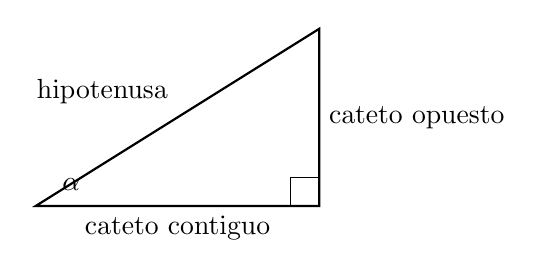
\begin{tikzpicture}[scale=0.9]
  \draw[thick] (0,0) -- (4,0) -- (4,2.5) -- cycle;
  \draw (3.6,0) -- (3.6,0.4) -- (4,0.4);
  \node[below] at (2,0) {cateto contiguo};
  \node[right] at (4,1.25) {cateto opuesto};
  \node[above left] at (2,1.3) {hipotenusa};
  \node at (0.5,0.3) {\(\alpha\)};
\end{tikzpicture}
\end{center}
\end{theorybox}

\begin{methodbox}{Como reconocer y resolver}
\begin{enumerate}
  \item Busca un triangulo rectangulo dentro de la figura.
  \item Elige la razon que relaciona el dato conocido con el buscado.
  \item Si la figura no es un triangulo, traza alturas o diagonales para dividirla.
\end{enumerate}
\end{methodbox}

\begin{solvedexample}{[EX-C05.S02-01] Triangulo isosceles resuelto por descomposicion}
Un triangulo isosceles tiene lados iguales de \(\SI{10}{cm}\) y angulo del vertice
\(120^\circ\). Calcula la base y el area.

\textbf{Desarrollo.} La altura desde el vertice parte el triangulo en dos triangulos
rectangulos con hipotenusa \(\SI{10}{cm}\) y angulo \(60^\circ\).

La mitad de la base vale
\[
10\sen 60^\circ=10\cdot \frac{\sqrt{3}}{2}=5\sqrt{3}.
\]
Luego la base completa es
\[
b=10\sqrt{3}\text{ cm}.
\]
La altura vale
\[
h=10\cos 60^\circ=10\cdot \frac{1}{2}=5\text{ cm}.
\]
Por tanto,
\[
A=\frac{b\cdot h}{2}=\frac{10\sqrt{3}\cdot 5}{2}=25\sqrt{3}\text{ cm}^2.
\]

\textbf{Respuesta final.}
\[
b=10\sqrt{3}\text{ cm},
\qquad
A=25\sqrt{3}\text{ cm}^2.
\]
\end{solvedexample}

\begin{commonerror}{Confundir el angulo entero con el semangulo}
Cuando una altura divide un triangulo isosceles, el angulo del vertice tambien se parte en dos.
Si se sigue usando \(120^\circ\) dentro del triangulo rectangulo, toda la razon queda mal.
\end{commonerror}

\begin{guidedexercise}{[GX-C05.S02-01] Catetos desde la hipotenusa}
En un triangulo rectangulo la hipotenusa mide \(\SI{10}{cm}\) y uno de los angulos agudos es
\(30^\circ\). Halla los dos catetos.

\textbf{Pista 1.} Usa \(\sen 30^\circ\) y \(\cos 30^\circ\).
\end{guidedexercise}

\begin{shortanswer}{[GX-C05.S02-01]}
Catetos: \(\SI{5}{cm}\) y \(5\sqrt{3}\,\si{cm}\).
\end{shortanswer}

\begin{fullsolution}{[GX-C05.S02-01]}
\[
\text{opuesto}=10\sen 30^\circ=5,
\qquad
\text{contiguo}=10\cos 30^\circ=5\sqrt{3}.
\]
\end{fullsolution}

\begin{guidedexercise}{[GX-C05.S02-02] Cateto e hipotenusa}
En un triangulo rectangulo, el cateto contiguo a un angulo de \(45^\circ\) mide \(\SI{6}{cm}\).
Halla la hipotenusa y el otro cateto.

\textbf{Pista 1.} En \(45^\circ\), \(\tg 45^\circ=1\).
\end{guidedexercise}

\begin{shortanswer}{[GX-C05.S02-02]}
Hipotenusa: \(6\sqrt{2}\,\si{cm}\). Otro cateto: \(\SI{6}{cm}\).
\end{shortanswer}

\begin{fullsolution}{[GX-C05.S02-02]}
Si el angulo es \(45^\circ\), ambos catetos coinciden. Luego el otro cateto tambien mide
\(\SI{6}{cm}\). Por Pitagoras,
\[
h=\sqrt{6^2+6^2}=6\sqrt{2}.
\]
\end{fullsolution}

\subsection*{Practica autonoma graduada}
\begin{exercise}{[PX-C05.S02-01] En un triangulo rectangulo, el cateto opuesto a \(30^\circ\) mide \(\SI{4}{cm}\). Halla la hipotenusa y el otro cateto.}
\end{exercise}
\begin{exercise}{[PX-C05.S02-02] En un triangulo rectangulo, la hipotenusa mide \(\SI{12}{cm}\) y un angulo agudo es \(60^\circ\). Halla los catetos.}
\end{exercise}
\begin{exercise}{[PX-C05.S02-03] Un triangulo isosceles tiene lados iguales de \(\SI{10}{cm}\) y angulo del vertice \(120^\circ\). Halla la base.}
\end{exercise}
\begin{exercise}{[PX-C05.S02-04] Un rombo tiene lado \(\SI{8}{cm}\) y angulo agudo \(60^\circ\). Halla sus diagonales.}
\end{exercise}
\begin{exercise}{[PX-C05.S02-05] Un hexagono regular tiene lado \(\SI{4}{cm}\). Halla su apotema.}
\end{exercise}
\begin{exercise}{[PX-C05.S02-06] Un rectangulo tiene diagonal \(\SI{10}{cm}\) y la diagonal forma \(30^\circ\) con la base. Halla las longitudes de base y altura.}
\end{exercise}

\begin{shortanswer}{C05.S02 practica autonoma}
\begin{enumerate}[label=\textbf{PX-C05.S02-\arabic*:}, leftmargin=*]
  \item Hipotenusa: \(\SI{8}{cm}\). Otro cateto: \(4\sqrt{3}\,\si{cm}\)
  \item Catetos: \(\SI{6}{cm}\) y \(6\sqrt{3}\,\si{cm}\)
  \item \(10\sqrt{3}\,\si{cm}\)
  \item \(\SI{8}{cm}\) y \(8\sqrt{3}\,\si{cm}\)
  \item \(2\sqrt{3}\,\si{cm}\)
  \item Base: \(5\sqrt{3}\,\si{cm}\). Altura: \(\SI{5}{cm}\)
\end{enumerate}
\end{shortanswer}

\begin{fullsolution}{C05.S02 practica autonoma}
\begin{enumerate}[label=\textbf{PX-C05.S02-\arabic*:}, leftmargin=*]
  \item \(\sen 30^\circ=\frac{4}{h}\), luego \(h=8\). El otro cateto es \(8\cos 30^\circ=4\sqrt{3}\).
  \item \(12\cos 60^\circ=6\) y \(12\sen 60^\circ=6\sqrt{3}\).
  \item Es el mismo calculo del ejemplo: la base vale \(10\sqrt{3}\).
  \item Las semidiagonales forman triangulos rectangulos: \(d_1=8\) y \(d_2=8\sqrt{3}\).
  \item En el triangulo central, la apotema es \(4\cos 30^\circ=2\sqrt{3}\).
  \item Base \(=10\cos 30^\circ=5\sqrt{3}\) y altura \(=10\sen 30^\circ=5\).
\end{enumerate}
\end{fullsolution}

\section{[C05.S03] Angulos notables y reduccion al primer cuadrante}

\subsection*{Objetivos de aprendizaje}
\begin{itemize}
  \item Hallar razones trigonometricas exactas en angulos relacionados.
  \item Controlar el signo correcto segun el cuadrante.
\end{itemize}

\subsection*{Prerrequisitos}
\begin{itemize}
  \item Conversion entre grados y radianes.
\end{itemize}

\begin{theorybox}{Idea minima}
Los angulos notables \(30^\circ\), \(45^\circ\) y \(60^\circ\) generan valores exactos. Para un
angulo cualquiera, se puede reducir al primer cuadrante y decidir el signo por cuadrantes.

\begin{center}
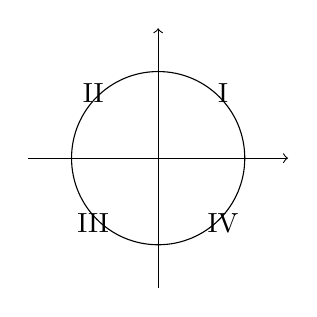
\begin{tikzpicture}[scale=1.1]
  \draw[->] (-1.5,0) -- (1.5,0);
  \draw[->] (0,-1.5) -- (0,1.5);
  \draw (0,0) circle (1);
  \node at (0.75,0.75) {I};
  \node at (-0.75,0.75) {II};
  \node at (-0.75,-0.75) {III};
  \node at (0.75,-0.75) {IV};
\end{tikzpicture}
\end{center}
\end{theorybox}

\begin{methodbox}{Como reconocer y resolver}
\begin{enumerate}
  \item Reduce el angulo a otro coterminal si supera una vuelta.
  \item Busca el angulo de referencia en el primer cuadrante.
  \item Asigna el signo correcto segun el cuadrante.
\end{enumerate}
\end{methodbox}

\begin{solvedexample}{[EX-C05.S03-01] Valores exactos por cuadrantes}
Calcula \(\sen 150^\circ\), \(\cos 240^\circ\) y \(\tg 330^\circ\).

\textbf{Desarrollo.}
\[
\sen 150^\circ=\sen(180^\circ-30^\circ)=\sen 30^\circ=\frac{1}{2}.
\]
\[
\cos 240^\circ=\cos(180^\circ+60^\circ)=-\cos 60^\circ=-\frac{1}{2}.
\]
\[
\tg 330^\circ=\tg(360^\circ-30^\circ)=-\tg 30^\circ=-\frac{\sqrt{3}}{3}.
\]

\textbf{Respuesta final.}
\[
\sen 150^\circ=\frac{1}{2},
\qquad
\cos 240^\circ=-\frac{1}{2},
\qquad
\tg 330^\circ=-\frac{\sqrt{3}}{3}.
\]
\end{solvedexample}

\begin{commonerror}{Conservar siempre el mismo signo}
El angulo de referencia da el valor absoluto, pero el signo no se conserva siempre. Hay que
mirar en que cuadrante cae el angulo original.
\end{commonerror}

\begin{guidedexercise}{[GX-C05.S03-01] Seno en el segundo cuadrante}
Calcula \(\sen 120^\circ\).

\textbf{Pista 1.} Usa \(120^\circ=180^\circ-60^\circ\).
\end{guidedexercise}

\begin{shortanswer}{[GX-C05.S03-01]}
\[
\sen 120^\circ=\frac{\sqrt{3}}{2}.
\]
\end{shortanswer}

\begin{fullsolution}{[GX-C05.S03-01]}
\[
\sen 120^\circ=\sen(180^\circ-60^\circ)=\sen 60^\circ=\frac{\sqrt{3}}{2}.
\]
\end{fullsolution}

\begin{guidedexercise}{[GX-C05.S03-02] Coseno en el cuarto cuadrante}
Calcula \(\cos 300^\circ\).

\textbf{Pista 1.} Usa \(300^\circ=360^\circ-60^\circ\).
\end{guidedexercise}

\begin{shortanswer}{[GX-C05.S03-02]}
\[
\cos 300^\circ=\frac{1}{2}.
\]
\end{shortanswer}

\begin{fullsolution}{[GX-C05.S03-02]}
\[
\cos 300^\circ=\cos(360^\circ-60^\circ)=\cos 60^\circ=\frac{1}{2}.
\]
\end{fullsolution}

\subsection*{Practica autonoma graduada}
\begin{exercise}{[PX-C05.S03-01] Calcula \(\cos 135^\circ\).}
\end{exercise}
\begin{exercise}{[PX-C05.S03-02] Calcula \(\sen 225^\circ\).}
\end{exercise}
\begin{exercise}{[PX-C05.S03-03] Calcula \(\tg 150^\circ\).}
\end{exercise}
\begin{exercise}{[PX-C05.S03-04] Calcula \(\cos 330^\circ\).}
\end{exercise}
\begin{exercise}{[PX-C05.S03-05] Calcula \(\sen 600^\circ\).}
\end{exercise}
\begin{exercise}{[PX-C05.S03-06] Calcula \(\tg 210^\circ\).}
\end{exercise}

\begin{shortanswer}{C05.S03 practica autonoma}
\begin{enumerate}[label=\textbf{PX-C05.S03-\arabic*:}, leftmargin=*]
  \item \(-\frac{\sqrt{2}}{2}\)
  \item \(-\frac{\sqrt{2}}{2}\)
  \item \(-\frac{\sqrt{3}}{3}\)
  \item \(\frac{\sqrt{3}}{2}\)
  \item \(-\frac{\sqrt{3}}{2}\)
  \item \(\frac{\sqrt{3}}{3}\)
\end{enumerate}
\end{shortanswer}

\begin{fullsolution}{C05.S03 practica autonoma}
\begin{enumerate}[label=\textbf{PX-C05.S03-\arabic*:}, leftmargin=*]
  \item \(\cos 135^\circ=\cos(180^\circ-45^\circ)=-\cos 45^\circ\).
  \item \(\sen 225^\circ=\sen(180^\circ+45^\circ)=-\sen 45^\circ\).
  \item \(\tg 150^\circ=\tg(180^\circ-30^\circ)=-\tg 30^\circ\).
  \item \(\cos 330^\circ=\cos(360^\circ-30^\circ)=\cos 30^\circ\).
  \item \(600^\circ=240^\circ\), luego \(\sen 600^\circ=\sen 240^\circ=-\sen 60^\circ\).
  \item \(\tg 210^\circ=\tg(180^\circ+30^\circ)=\tg 30^\circ\).
\end{enumerate}
\end{fullsolution}

\section{[C05.S04] Calculo de razones a partir de una razon conocida}

\subsection*{Objetivos de aprendizaje}
\begin{itemize}
  \item Reconstruir las razones restantes a partir de una sola.
  \item Combinar Pitagoras trigonometrico y signos por cuadrantes.
\end{itemize}

\subsection*{Prerrequisitos}
\begin{itemize}
  \item Angulos notables, reduccion y fracciones.
\end{itemize}

\begin{theorybox}{Idea minima}
Si conoces una razon trigonometrica y el cuadrante, puedes reconstruir un triangulo auxiliar y
hallar las demas. La identidad basica es
\[
\sen^2 x+\cos^2 x=1.
\]
\end{theorybox}

\begin{methodbox}{Como reconocer y resolver}
\begin{enumerate}
  \item Dibuja un triangulo o usa la identidad \(\sen^2 x+\cos^2 x=1\).
  \item Decide el signo de cada razon con el cuadrante.
  \item Calcula despues \(\tg x=\frac{\sen x}{\cos x}\).
\end{enumerate}
\end{methodbox}

\begin{solvedexample}{[EX-C05.S04-01] Una razon y el cuadrante}
Sabiendo que \(\sen x=\frac{3}{5}\) y que \(x\) esta en el segundo cuadrante, calcula
\(\cos x\) y \(\tg x\).

\textbf{Desarrollo.} Si \(\sen x=\frac{3}{5}\), tomamos cateto opuesto \(3\) e hipotenusa \(5\).
Entonces el cateto contiguo tiene modulo
\[
\sqrt{5^2-3^2}=4.
\]
En el segundo cuadrante el coseno es negativo, asi que
\[
\cos x=-\frac{4}{5}.
\]
Luego
\[
\tg x=\frac{\sen x}{\cos x}=\frac{3/5}{-4/5}=-\frac{3}{4}.
\]

\textbf{Respuesta final.}
\[
\cos x=-\frac{4}{5},
\qquad
\tg x=-\frac{3}{4}.
\]
\end{solvedexample}

\begin{commonerror}{Perder el signo del cuadrante}
El triangulo auxiliar da modulos positivos. El signo final no sale del triangulo, sino del
cuadrante en que esta el angulo.
\end{commonerror}

\begin{guidedexercise}{[GX-C05.S04-01] Coseno conocido en el tercer cuadrante}
Si \(\cos x=-\frac{12}{13}\) y \(x\) esta en el tercer cuadrante, calcula \(\sen x\) y
\(\tg x\).

\textbf{Pista 1.} La hipotenusa es \(13\) y el otro cateto tiene modulo \(5\).
\end{guidedexercise}

\begin{shortanswer}{[GX-C05.S04-01]}
\[
\sen x=-\frac{5}{13},
\qquad
\tg x=\frac{5}{12}.
\]
\end{shortanswer}

\begin{fullsolution}{[GX-C05.S04-01]}
Por Pitagoras, el cateto restante vale \(5\). En el tercer cuadrante, seno y coseno son
negativos y la tangente es positiva:
\[
\sen x=-\frac{5}{13},
\qquad
\tg x=\frac{-5/13}{-12/13}=\frac{5}{12}.
\]
\end{fullsolution}

\begin{guidedexercise}{[GX-C05.S04-02] Tangente conocida en el cuarto cuadrante}
Si \(\tg x=-2\) y \(x\) esta en el cuarto cuadrante, calcula \(\sen x\) y \(\cos x\).

\textbf{Pista 1.} Puedes tomar catetos de modulos \(2\) y \(1\).
\end{guidedexercise}

\begin{shortanswer}{[GX-C05.S04-02]}
\[
\sen x=-\frac{2\sqrt{5}}{5},
\qquad
\cos x=\frac{\sqrt{5}}{5}.
\]
\end{shortanswer}

\begin{fullsolution}{[GX-C05.S04-02]}
Si \(\tg x=-2\), podemos tomar cateto opuesto \(-2\) y contiguo \(1\). La hipotenusa es
\(\sqrt{5}\), luego
\[
\sen x=-\frac{2}{\sqrt{5}}=-\frac{2\sqrt{5}}{5},
\qquad
\cos x=\frac{1}{\sqrt{5}}=\frac{\sqrt{5}}{5}.
\]
\end{fullsolution}

\subsection*{Practica autonoma graduada}
\begin{exercise}{[PX-C05.S04-01] Si \(\cos x=\frac{5}{13}\) y \(x\) esta en el primer cuadrante, calcula \(\sen x\) y \(\tg x\).}
\end{exercise}
\begin{exercise}{[PX-C05.S04-02] Si \(\sen x=-\frac{4}{5}\) y \(x\) esta en el cuarto cuadrante, calcula \(\cos x\) y \(\tg x\).}
\end{exercise}
\begin{exercise}{[PX-C05.S04-03] Si \(\tg x=\frac{3}{4}\) y \(x\) esta en el tercer cuadrante, calcula \(\sen x\) y \(\cos x\).}
\end{exercise}
\begin{exercise}{[PX-C05.S04-04] Si \(\cos x=-\frac{8}{17}\) y \(x\) esta en el segundo cuadrante, calcula \(\sen x\) y \(\tg x\).}
\end{exercise}
\begin{exercise}{[PX-C05.S04-05] Si \(\sen x=\frac{12}{13}\) y \(x\) esta en el primer cuadrante, calcula \(\cos x\) y \(\tg x\).}
\end{exercise}
\begin{exercise}{[PX-C05.S04-06] Si \(\tg x=-1\) y \(x\) esta en el segundo cuadrante, calcula \(\sen x\) y \(\cos x\).}
\end{exercise}

\begin{shortanswer}{C05.S04 practica autonoma}
\begin{enumerate}[label=\textbf{PX-C05.S04-\arabic*:}, leftmargin=*]
  \item \(\sen x=\frac{12}{13}\), \(\tg x=\frac{12}{5}\)
  \item \(\cos x=\frac{3}{5}\), \(\tg x=-\frac{4}{3}\)
  \item \(\sen x=-\frac{3}{5}\), \(\cos x=-\frac{4}{5}\)
  \item \(\sen x=\frac{15}{17}\), \(\tg x=-\frac{15}{8}\)
  \item \(\cos x=\frac{5}{13}\), \(\tg x=\frac{12}{5}\)
  \item \(\sen x=\frac{\sqrt{2}}{2}\), \(\cos x=-\frac{\sqrt{2}}{2}\)
\end{enumerate}
\end{shortanswer}

\begin{fullsolution}{C05.S04 practica autonoma}
\begin{enumerate}[label=\textbf{PX-C05.S04-\arabic*:}, leftmargin=*]
  \item Es un triangulo \(5\)-\(12\)-\(13\), todo positivo en el primer cuadrante.
  \item Si el seno es \(-\frac{4}{5}\), el coseno tiene modulo \(\frac{3}{5}\) y es positivo.
  \item Para \(\tg x=\frac{3}{4}\) en el tercer cuadrante, seno y coseno son negativos.
  \item Es un triangulo \(8\)-\(15\)-\(17\) y en el segundo cuadrante la tangente es negativa.
  \item El cateto restante vale \(5\), con todo positivo.
  \item Si \(|\tg x|=1\), los catetos tienen igual modulo. En el segundo cuadrante el seno es
  positivo y el coseno negativo.
\end{enumerate}
\end{fullsolution}

\section{[C05.S05] Identidades y transformaciones trigonometricas}

\subsection*{Objetivos de aprendizaje}
\begin{itemize}
  \item Aplicar identidades fundamentales y de angulos relacionados.
  \item Calcular razones de angulo doble sin recurrir a calculadora.
\end{itemize}

\subsection*{Prerrequisitos}
\begin{itemize}
  \item Razones de un angulo conocido y signos por cuadrantes.
\end{itemize}

\begin{theorybox}{Idea minima}
Las identidades mas usadas en este nivel son
\[
\sen^2 x+\cos^2 x=1,
\qquad
\sen(2x)=2\sen x\cos x,
\qquad
\cos(2x)=\cos^2 x-\sen^2 x.
\]
Tambien conviene recordar
\[
\sen(\pi-x)=\sen x,
\qquad
\cos(\pi+x)=-\cos x.
\]
\end{theorybox}

\begin{methodbox}{Como reconocer y resolver}
\begin{enumerate}
  \item Reescribe primero todo con \(\sen x\), \(\cos x\) y \(\tg x\).
  \item Usa el cuadrante para fijar signos.
  \item Sustituye al final en la identidad elegida.
\end{enumerate}
\end{methodbox}

\begin{solvedexample}{[EX-C05.S05-01] Angulo doble a partir de un dato}
Si \(\sen x=\frac{4}{5}\) y \(x\) esta en el primer cuadrante, calcula \(\cos x\), \(\tg x\),
\(\sen 2x\) y \(\cos 2x\).

\textbf{Desarrollo.} Por Pitagoras trigonometrico,
\[
\cos x=\frac{3}{5},
\qquad
\tg x=\frac{4/5}{3/5}=\frac{4}{3}.
\]
Ahora aplicamos las formulas de angulo doble:
\[
\sen 2x=2\sen x\cos x=2\cdot \frac{4}{5}\cdot \frac{3}{5}=\frac{24}{25},
\]
\[
\cos 2x=\cos^2 x-\sen^2 x=\frac{9}{25}-\frac{16}{25}=-\frac{7}{25}.
\]

\textbf{Respuesta final.}
\[
\cos x=\frac{3}{5},
\quad
\tg x=\frac{4}{3},
\quad
\sen 2x=\frac{24}{25},
\quad
\cos 2x=-\frac{7}{25}.
\]
\end{solvedexample}

\begin{commonerror}{Cambiar de identidad a mitad del calculo}
Si ya has hallado \(\sen x\) y \(\cos x\), lo mas seguro es sustituirlos en una formula clara.
Intentar mezclar varias identidades sin orden suele introducir errores de signo.
\end{commonerror}

\begin{guidedexercise}{[GX-C05.S05-01] Identidad fundamental}
Simplifica \(\sen^2 x+\cos^2 x\).

\textbf{Pista 1.} Es una identidad basica.
\end{guidedexercise}

\begin{shortanswer}{[GX-C05.S05-01]}
\[
\sen^2 x+\cos^2 x=1.
\]
\end{shortanswer}

\begin{fullsolution}{[GX-C05.S05-01]}
Directamente por la identidad fundamental:
\[
\sen^2 x+\cos^2 x=1.
\]
\end{fullsolution}

\begin{guidedexercise}{[GX-C05.S05-02] Producto seno por coseno}
Si \(\tg x=2\) y \(x\) esta en el primer cuadrante, calcula \(\sen x\cos x\).

\textbf{Pista 1.} Toma un triangulo con catetos \(2\) y \(1\).
\end{guidedexercise}

\begin{shortanswer}{[GX-C05.S05-02]}
\[
\sen x\cos x=\frac{2}{5}.
\]
\end{shortanswer}

\begin{fullsolution}{[GX-C05.S05-02]}
Con catetos \(2\) y \(1\), la hipotenusa es \(\sqrt{5}\). Entonces
\[
\sen x=\frac{2}{\sqrt{5}},
\qquad
\cos x=\frac{1}{\sqrt{5}},
\]
y por tanto
\[
\sen x\cos x=\frac{2}{5}.
\]
\end{fullsolution}

\subsection*{Practica autonoma graduada}
\begin{exercise}{[PX-C05.S05-01] Si \(\cos x=\frac{12}{13}\) y \(x\) esta en el primer cuadrante, calcula \(\sen 2x\).}
\end{exercise}
\begin{exercise}{[PX-C05.S05-02] Si \(\sen x=\frac{5}{13}\) y \(x\) esta en el primer cuadrante, calcula \(\cos 2x\).}
\end{exercise}
\begin{exercise}{[PX-C05.S05-03] Simplifica \(\sen(\pi-x)\).}
\end{exercise}
\begin{exercise}{[PX-C05.S05-04] Simplifica \(\cos(\pi+x)\).}
\end{exercise}
\begin{exercise}{[PX-C05.S05-05] Si \(\tg x=\frac{3}{4}\) y \(x\) esta en el primer cuadrante, calcula \(\tg 2x\).}
\end{exercise}
\begin{exercise}{[PX-C05.S05-06] Si \(\sen x=\frac{3}{5}\) y \(x\) esta en el segundo cuadrante, calcula \(\cos 2x\).}
\end{exercise}

\begin{shortanswer}{C05.S05 practica autonoma}
\begin{enumerate}[label=\textbf{PX-C05.S05-\arabic*:}, leftmargin=*]
  \item \(\frac{120}{169}\)
  \item \(\frac{119}{169}\)
  \item \(\sen x\)
  \item \(-\cos x\)
  \item \(\frac{24}{7}\)
  \item \(\frac{7}{25}\)
\end{enumerate}
\end{shortanswer}

\begin{fullsolution}{C05.S05 practica autonoma}
\begin{enumerate}[label=\textbf{PX-C05.S05-\arabic*:}, leftmargin=*]
  \item El seno vale \(\frac{5}{13}\). Luego \(\sen 2x=2\cdot \frac{5}{13}\cdot \frac{12}{13}=\frac{120}{169}\).
  \item \(\cos 2x=1-2\sen^2 x=1-2\cdot \frac{25}{169}=\frac{119}{169}\).
  \item \(\sen(\pi-x)=\sen x\).
  \item \(\cos(\pi+x)=-\cos x\).
  \item \(\tg 2x=\frac{2\tg x}{1-\tg^2 x}=\frac{2\cdot 3/4}{1-9/16}=\frac{24}{7}\).
  \item Aunque \(\cos x\) sea negativo en el segundo cuadrante, \(\cos 2x\) depende de los cuadrados:
  \(\cos 2x=\frac{16}{25}-\frac{9}{25}=\frac{7}{25}\).
\end{enumerate}
\end{fullsolution}

\section{[C05.S06] Ecuaciones trigonometricas}

\subsection*{Objetivos de aprendizaje}
\begin{itemize}
  \item Resolver ecuaciones trigonometricas elementales.
  \item Expresar soluciones generales con \(k\in\mathbb{Z}\).
\end{itemize}

\subsection*{Prerrequisitos}
\begin{itemize}
  \item Angulos notables y periodicidad de seno, coseno y tangente.
\end{itemize}

\begin{theorybox}{Idea minima}
Las funciones trigonometricas son periodicas:
\[
\sen(x+2\pi)=\sen x,
\qquad
\cos(x+2\pi)=\cos x,
\qquad
\tg(x+\pi)=\tg x.
\]
Por eso una ecuacion trigonometrica suele tener infinitas soluciones y conviene escribir la
familia general.
\end{theorybox}

\begin{methodbox}{Como reconocer y resolver}
\begin{enumerate}
  \item Encuentra primero las soluciones en un intervalo base, por ejemplo \([0,2\pi)\).
  \item Usa el periodo adecuado para escribir la solucion general.
  \item Comprueba si la funcion es seno, coseno o tangente antes de elegir el periodo.
\end{enumerate}
\end{methodbox}

\begin{solvedexample}{[EX-C05.S06-01] Seno igual a un valor notable}
Resuelve \(\sen x=\frac{1}{2}\).

\textbf{Desarrollo.} En \([0,2\pi)\), el seno vale \(\frac{1}{2}\) en
\[
x=\frac{\pi}{6}
\qquad \text{y} \qquad
x=\frac{5\pi}{6}.
\]
Como el seno tiene periodo \(2\pi\), las soluciones generales son
\[
x=\frac{\pi}{6}+2k\pi
\qquad \text{o} \qquad
x=\frac{5\pi}{6}+2k\pi,
\qquad k\in\mathbb{Z}.
\]

\textbf{Respuesta final.}
\[
x=\frac{\pi}{6}+2k\pi
\quad \text{o} \quad
x=\frac{5\pi}{6}+2k\pi,
\qquad k\in\mathbb{Z}.
\]
\end{solvedexample}

\begin{commonerror}{Usar siempre el mismo periodo}
El seno y el coseno repiten cada \(2\pi\), pero la tangente repite cada \(\pi\). Si se usa
\(2\pi\) para todo, algunas soluciones quedan incompletas.
\end{commonerror}

\begin{guidedexercise}{[GX-C05.S06-01] Coseno negativo}
Resuelve \(\cos x=-\frac{\sqrt{2}}{2}\).

\textbf{Pista 1.} Busca primero los angulos de referencia de \(45^\circ\).
\end{guidedexercise}

\begin{shortanswer}{[GX-C05.S06-01]}
\[
x=\frac{3\pi}{4}+2k\pi
\quad \text{o} \quad
x=\frac{5\pi}{4}+2k\pi,
\qquad k\in\mathbb{Z}.
\]
\end{shortanswer}

\begin{fullsolution}{[GX-C05.S06-01]}
En \([0,2\pi)\), el coseno vale \(-\frac{\sqrt{2}}{2}\) en
\[
\frac{3\pi}{4}
\qquad \text{y} \qquad
\frac{5\pi}{4}.
\]
Al tener periodo \(2\pi\), se anade \(2k\pi\).
\end{fullsolution}

\begin{guidedexercise}{[GX-C05.S06-02] Tangente nula}
Resuelve \(\tg x=0\).

\textbf{Pista 1.} Piensa en los multiplos de \(\pi\).
\end{guidedexercise}

\begin{shortanswer}{[GX-C05.S06-02]}
\[
x=k\pi,
\qquad k\in\mathbb{Z}.
\]
\end{shortanswer}

\begin{fullsolution}{[GX-C05.S06-02]}
La tangente es \(0\) cuando el seno es \(0\) y el coseno no lo es. Eso ocurre en
\[
x=0,\pi,2\pi,\ldots
\]
y la forma general es \(x=k\pi\).
\end{fullsolution}

\subsection*{Practica autonoma graduada}
\begin{exercise}{[PX-C05.S06-01] Resuelve \(\cos x=0\).}
\end{exercise}
\begin{exercise}{[PX-C05.S06-02] Resuelve \(\tg x=1\).}
\end{exercise}
\begin{exercise}{[PX-C05.S06-03] Resuelve \(\sen x=-1\).}
\end{exercise}
\begin{exercise}{[PX-C05.S06-04] Resuelve \(\cos x=\frac{\sqrt{2}}{2}\).}
\end{exercise}
\begin{exercise}{[PX-C05.S06-05] Resuelve \(\sen x=\frac{\sqrt{3}}{2}\).}
\end{exercise}
\begin{exercise}{[PX-C05.S06-06] Resuelve \(\tg x=-\sqrt{3}\).}
\end{exercise}

\begin{shortanswer}{C05.S06 practica autonoma}
\begin{enumerate}[label=\textbf{PX-C05.S06-\arabic*:}, leftmargin=*]
  \item \(x=\frac{\pi}{2}+k\pi\)
  \item \(x=\frac{\pi}{4}+k\pi\)
  \item \(x=\frac{3\pi}{2}+2k\pi\)
  \item \(x=\frac{\pi}{4}+2k\pi\) o \(x=\frac{7\pi}{4}+2k\pi\)
  \item \(x=\frac{\pi}{3}+2k\pi\) o \(x=\frac{2\pi}{3}+2k\pi\)
  \item \(x=-\frac{\pi}{3}+k\pi\)
\end{enumerate}
\end{shortanswer}

\begin{fullsolution}{C05.S06 practica autonoma}
\begin{enumerate}[label=\textbf{PX-C05.S06-\arabic*:}, leftmargin=*]
  \item En \([0,2\pi)\), las soluciones son \(\frac{\pi}{2}\) y \(\frac{3\pi}{2}\), que se
  agrupan como \(\frac{\pi}{2}+k\pi\).
  \item La tangente vale \(1\) en \(\frac{\pi}{4}\) y repite cada \(\pi\).
  \item El seno solo vale \(-1\) en \(\frac{3\pi}{2}\) mas vueltas completas.
  \item El coseno es \(\frac{\sqrt{2}}{2}\) en los cuadrantes I y IV.
  \item El seno es \(\frac{\sqrt{3}}{2}\) en los cuadrantes I y II.
  \item La tangente vale \(-\sqrt{3}\) con angulo de referencia \(\frac{\pi}{3}\) y periodo \(\pi\).
\end{enumerate}
\end{fullsolution}

\section{[C05.S07] Resolucion de triangulos}

\subsection*{Objetivos de aprendizaje}
\begin{itemize}
  \item Resolver triangulos oblicuangulos sencillos.
  \item Escoger entre teorema del seno y teorema del coseno.
\end{itemize}

\subsection*{Prerrequisitos}
\begin{itemize}
  \item Razones trigonometricas y angulos interiores de un triangulo.
\end{itemize}

\begin{theorybox}{Idea minima}
En cualquier triangulo \(ABC\), con lados opuestos \(a\), \(b\) y \(c\),
\[
\frac{a}{\sen A}=\frac{b}{\sen B}=\frac{c}{\sen C}
\]
y
\[
a^2=b^2+c^2-2bc\cos A.
\]
El teorema del seno es muy util en casos ALA o AAL; el del coseno, en casos LAL o LLL.
\end{theorybox}

\begin{methodbox}{Como reconocer y resolver}
\begin{enumerate}
  \item Si conoces dos angulos y un lado, empieza por el teorema del seno.
  \item Si conoces dos lados y el angulo comprendido, usa el teorema del coseno.
  \item Comprueba al final que la suma de angulos es \(180^\circ\).
\end{enumerate}
\end{methodbox}

\begin{solvedexample}{[EX-C05.S07-01] Resolver un triangulo con dos angulos}
En un triangulo \(ABC\), se sabe que \(A=30^\circ\), \(B=60^\circ\) y \(a=\SI{5}{cm}\).
Calcula \(C\), \(b\) y \(c\).

\textbf{Desarrollo.} La suma de angulos da
\[
C=180^\circ-30^\circ-60^\circ=90^\circ.
\]
Aplicamos ahora el teorema del seno:
\[
\frac{a}{\sen A}=\frac{b}{\sen B}=\frac{c}{\sen C}.
\]
Como
\[
\frac{5}{\sen 30^\circ}=\frac{5}{1/2}=10,
\]
se obtiene
\[
b=10\sen 60^\circ=10\cdot \frac{\sqrt{3}}{2}=5\sqrt{3},
\qquad
c=10\sen 90^\circ=10.
\]

\textbf{Respuesta final.}
\[
C=90^\circ,
\qquad
b=5\sqrt{3}\text{ cm},
\qquad
c=\SI{10}{cm}.
\]
\end{solvedexample}

\begin{commonerror}{Aplicar el seno sin emparejar lado y angulo opuestos}
En el teorema del seno cada lado debe ir con su angulo opuesto. Mezclar correspondencias lleva
a ecuaciones incorrectas aunque las razones parezcan parecidas.
\end{commonerror}

\begin{guidedexercise}{[GX-C05.S07-01] Angulo recto conocido}
En un triangulo, \(A=30^\circ\), \(B=90^\circ\) y \(a=\SI{8}{cm}\). Halla \(b\).

\textbf{Pista 1.} Primero calcula \(\frac{a}{\sen A}\).
\end{guidedexercise}

\begin{shortanswer}{[GX-C05.S07-01]}
\[
b=\SI{16}{cm}.
\]
\end{shortanswer}

\begin{fullsolution}{[GX-C05.S07-01]}
\[
\frac{a}{\sen A}=\frac{8}{1/2}=16.
\]
Como \(\sen 90^\circ=1\), se sigue que \(b=16\).
\end{fullsolution}

\begin{guidedexercise}{[GX-C05.S07-02] Dos lados y angulo comprendido}
Un triangulo tiene dos lados de \(\SI{5}{cm}\) y el angulo comprendido es \(60^\circ\). Halla
el tercer lado.

\textbf{Pista 1.} Usa el teorema del coseno.
\end{guidedexercise}

\begin{shortanswer}{[GX-C05.S07-02]}
\[
c=\SI{5}{cm}.
\]
\end{shortanswer}

\begin{fullsolution}{[GX-C05.S07-02]}
\[
c^2=5^2+5^2-2\cdot 5\cdot 5\cos 60^\circ=25+25-25=25.
\]
Luego \(c=5\).
\end{fullsolution}

\subsection*{Practica autonoma graduada}
\begin{exercise}{[PX-C05.S07-01] En un triangulo \(A=45^\circ\), \(B=45^\circ\) y \(a=\SI{4}{cm}\). Halla \(C\), \(b\) y \(c\).}
\end{exercise}
\begin{exercise}{[PX-C05.S07-02] En un triangulo \(A=30^\circ\), \(C=90^\circ\) y \(a=\SI{3}{cm}\). Halla \(B\), \(b\) y \(c\).}
\end{exercise}
\begin{exercise}{[PX-C05.S07-03] Un triangulo rectangulo tiene catetos \(\SI{6}{cm}\) y \(\SI{8}{cm}\). Halla la hipotenusa.}
\end{exercise}
\begin{exercise}{[PX-C05.S07-04] En un triangulo, \(a=\SI{5}{cm}\), \(b=\SI{5}{cm}\) y \(C=60^\circ\). Halla \(c\).}
\end{exercise}
\begin{exercise}{[PX-C05.S07-05] En un triangulo \(A=30^\circ\), \(B=60^\circ\) y \(a=\SI{4}{cm}\). Halla \(C\), \(b\) y \(c\).}
\end{exercise}
\begin{exercise}{[PX-C05.S07-06] En un triangulo rectangulo, la hipotenusa mide \(\SI{2}{cm}\) y uno de los angulos agudos es \(60^\circ\). Halla los catetos.}
\end{exercise}

\begin{shortanswer}{C05.S07 practica autonoma}
\begin{enumerate}[label=\textbf{PX-C05.S07-\arabic*:}, leftmargin=*]
  \item \(C=90^\circ\), \(b=\SI{4}{cm}\), \(c=4\sqrt{2}\,\si{cm}\)
  \item \(B=60^\circ\), \(b=3\sqrt{3}\,\si{cm}\), \(c=\SI{6}{cm}\)
  \item \(\SI{10}{cm}\)
  \item \(\SI{5}{cm}\)
  \item \(C=90^\circ\), \(b=4\sqrt{3}\,\si{cm}\), \(c=\SI{8}{cm}\)
  \item Catetos: \(\SI{1}{cm}\) y \(\sqrt{3}\,\si{cm}\)
\end{enumerate}
\end{shortanswer}

\begin{fullsolution}{C05.S07 practica autonoma}
\begin{enumerate}[label=\textbf{PX-C05.S07-\arabic*:}, leftmargin=*]
  \item Es un triangulo isosceles rectangulo: \(b=a=4\) y \(c=4\sqrt{2}\).
  \item \(B=60^\circ\). Con el teorema del seno, \(\frac{3}{\sen 30^\circ}=6\), luego \(b=6\sen 60^\circ=3\sqrt{3}\) y \(c=6\).
  \item Por Pitagoras, \(\sqrt{6^2+8^2}=10\).
  \item Teorema del coseno: \(c^2=25+25-50\cos 60^\circ=25\).
  \item Igual que el ejemplo, pero escalado: \(C=90^\circ\), \(b=4\sqrt{3}\), \(c=8\).
  \item El cateto opuesto a \(60^\circ\) vale \(2\sen 60^\circ=\sqrt{3}\) y el contiguo
  \(2\cos 60^\circ=1\).
\end{enumerate}
\end{fullsolution}

\section{[C05.S08] Problemas contextualizados de trigonometria}

\subsection*{Objetivos de aprendizaje}
\begin{itemize}
  \item Traducir un contexto real a un esquema trigonometrico.
  \item Responder con unidades y sentido geometrico.
\end{itemize}

\subsection*{Prerrequisitos}
\begin{itemize}
  \item Razones trigonometricas y teoremas del seno y del coseno.
\end{itemize}

\begin{theorybox}{Idea minima}
En problemas de alturas, distancias o navegacion, lo decisivo es construir el esquema correcto:
que lado representa cada magnitud, que angulo es de elevacion o de vision y que unidad debe
llevar la respuesta final.
\end{theorybox}

\begin{methodbox}{Como reconocer y resolver}
\begin{enumerate}
  \item Dibuja un esquema y marca con claridad los datos.
  \item Decide si el problema se reduce a un triangulo rectangulo o a un triangulo oblicuo.
  \item Resuelve y expresa la respuesta con unidades.
\end{enumerate}
\end{methodbox}

\begin{solvedexample}{[EX-C05.S08-01] Altura de una torre}
Dos puntos del suelo estan alineados con la base de una torre. El punto mas cercano observa la
cima con un angulo de elevacion de \(60^\circ\) y el mas lejano con un angulo de \(30^\circ\).
Entre ambos puntos hay \(\SI{20}{m}\). Halla la altura de la torre.

\textbf{Desarrollo.} Llamamos \(x\) a la distancia desde la base al punto cercano y \(h\) a la
altura.
\[
\tg 60^\circ=\frac{h}{x}
\qquad \Longrightarrow \qquad
h=x\sqrt{3}.
\]
Para el punto lejano, la distancia horizontal es \(x+20\):
\[
\tg 30^\circ=\frac{h}{x+20}=\frac{1}{\sqrt{3}}.
\]
Sustituyendo \(h=x\sqrt{3}\),
\[
\frac{x\sqrt{3}}{x+20}=\frac{1}{\sqrt{3}}
\qquad \Longrightarrow \qquad
3x=x+20
\qquad \Longrightarrow \qquad
x=10.
\]
Entonces
\[
h=10\sqrt{3}\text{ m}.
\]

\textbf{Respuesta final.}
\[
h=10\sqrt{3}\text{ m}.
\]
\end{solvedexample}

\begin{commonerror}{Usar la misma distancia horizontal dos veces}
Cada angulo se observa desde un punto distinto. Si se repite la misma distancia para ambos,
el planteamiento ya nace contradictorio.
\end{commonerror}

\begin{guidedexercise}{[GX-C05.S08-01] Distancia entre barcos}
Dos barcos salen del mismo puerto. Tras un tramo, uno esta a \(\SI{6}{km}\) del puerto y el
otro a \(\SI{8}{km}\), formando entre sus rumbos un angulo de \(60^\circ\). Halla la distancia
entre los barcos.

\textbf{Pista 1.} Usa el teorema del coseno.
\end{guidedexercise}

\begin{shortanswer}{[GX-C05.S08-01]}
\[
d=2\sqrt{13}\text{ km}.
\]
\end{shortanswer}

\begin{fullsolution}{[GX-C05.S08-01]}
\[
d^2=6^2+8^2-2\cdot 6\cdot 8\cos 60^\circ=36+64-48=52.
\]
Luego
\[
d=2\sqrt{13}\text{ km}.
\]
\end{fullsolution}

\begin{guidedexercise}{[GX-C05.S08-02] Altura desde un solo punto}
Desde un punto situado a \(\SI{12}{m}\) de la base de una farola se ve la parte alta con un
angulo de elevacion de \(45^\circ\). Halla la altura de la farola.

\textbf{Pista 1.} En \(45^\circ\), \(\tg 45^\circ=1\).
\end{guidedexercise}

\begin{shortanswer}{[GX-C05.S08-02]}
\[
h=\SI{12}{m}.
\]
\end{shortanswer}

\begin{fullsolution}{[GX-C05.S08-02]}
\[
\tg 45^\circ=\frac{h}{12}=1,
\]
de donde \(h=12\).
\end{fullsolution}

\subsection*{Practica autonoma graduada}
\begin{exercise}{[PX-C05.S08-01] Desde un punto a \(\SI{12}{m}\) de un poste se observa la parte alta con un angulo de \(45^\circ\). Halla la altura del poste.}
\end{exercise}
\begin{exercise}{[PX-C05.S08-02] Dos puntos alineados con la base de un edificio estan separados \(\SI{30}{m}\). Los angulos de elevacion a la azotea son \(60^\circ\) y \(30^\circ\). Halla la altura del edificio.}
\end{exercise}
\begin{exercise}{[PX-C05.S08-03] Dos barcos parten del mismo puerto. Tras cierto tiempo estan a \(\SI{20}{km}\) y \(\SI{30}{km}\) del puerto, con un angulo de \(60^\circ\) entre sus rumbos. Halla la distancia entre ellos.}
\end{exercise}
\begin{exercise}{[PX-C05.S08-04] En un parque triangular, dos lados miden \(\SI{6}{m}\) y \(\SI{10}{m}\), y el angulo comprendido es \(120^\circ\). Halla el tercer lado.}
\end{exercise}
\begin{exercise}{[PX-C05.S08-05] Un jugador esta a \(\SI{5}{m}\) de un poste y a \(\SI{8}{m}\) del otro. Si la distancia entre postes es \(\SI{7}{m}\), halla el angulo con el que ve la porteria.}
\end{exercise}
\begin{exercise}{[PX-C05.S08-06] Un cable llega a la parte alta de una pared de \(\SI{12}{m}\) y forma \(30^\circ\) con el suelo. Halla la longitud del cable.}
\end{exercise}

\begin{shortanswer}{C05.S08 practica autonoma}
\begin{enumerate}[label=\textbf{PX-C05.S08-\arabic*:}, leftmargin=*]
  \item \(\SI{12}{m}\)
  \item \(15\sqrt{3}\,\si{m}\)
  \item \(10\sqrt{7}\,\si{km}\)
  \item \(\SI{14}{m}\)
  \item \(60^\circ\)
  \item \(\SI{24}{m}\)
\end{enumerate}
\end{shortanswer}

\begin{fullsolution}{C05.S08 practica autonoma}
\begin{enumerate}[label=\textbf{PX-C05.S08-\arabic*:}, leftmargin=*]
  \item Igual que en el guiado: \(\tg 45^\circ=\frac{h}{12}\), luego \(h=12\).
  \item Si \(x\) es la distancia al punto cercano, \(\tg 60^\circ=\frac{h}{x}\) y
  \(\tg 30^\circ=\frac{h}{x+30}\). Sale \(x=15\) y por tanto \(h=15\sqrt{3}\).
  \item Por el teorema del coseno:
  \[
  d^2=20^2+30^2-2\cdot 20\cdot 30\cos 60^\circ=700.
  \]
  \item
  \[
  c^2=6^2+10^2-2\cdot 6\cdot 10\cos 120^\circ=36+100+60=196.
  \]
  \item El angulo \(\theta\) verifica
  \[
  \cos\theta=\frac{5^2+8^2-7^2}{2\cdot 5\cdot 8}=\frac{1}{2}.
  \]
  \item Si el cable forma \(30^\circ\) con el suelo, entonces
  \[
  \sen 30^\circ=\frac{12}{L}=\frac{1}{2},
  \]
  y por tanto \(L=24\).
\end{enumerate}
\end{fullsolution}

\begin{selfcheck}
\begin{itemize}
  \item Distingo cuando conviene trabajar en grados y cuando en radianes.
  \item Antes de operar con signos, localizo el cuadrante o el angulo de referencia.
  \item En ecuaciones trigonometricas, doy soluciones generales y no solo una vuelta.
  \item En problemas, dibujo un esquema y cuido las unidades de la respuesta final.
\end{itemize}
\end{selfcheck}

\begin{extension}{Exactitud frente a aproximacion}
En este bloque conviene conservar valores exactos mientras sea razonable: \(\sqrt{3}\),
\(\frac{\pi}{6}\), \(5\sqrt{3}\) o \(10\sqrt{7}\) comunican mejor la estructura del problema
que una aproximacion decimal prematura.
\end{extension}
